%%%%%%%%%%%%%%%%%%%%%%%%%%%%%%%%%%%%%%%%%%%%%%%%%%
%% Bachelor's & Master's Thesis Template        %%
%% Copyleft by Dawid Weiss & Marta Szachniuk    %%
%% Faculty of Computing and Telecommunication   %%
%% Poznan University of Technology, 2020        %%
%%%%%%%%%%%%%%%%%%%%%%%%%%%%%%%%%%%%%%%%%%%%%%%%%%


% Szkielet dla pracy licencjackiej pisanej w języku polskim.

\documentclass[polish,a4paper,oneside]{ppfcmthesis}


\usepackage[utf8]{inputenc}
\usepackage[OT4]{fontenc}

%--------------------------------------
% Strona tytułowa
%--------------------------------------

% Autorzy pracy, jeśli jest ich więcej niż jeden
% wstaw między nimi separator \and
\author{%
   Jakub Zdanowski \album{127239}
}
\authortitle{}                                % Do not change.

\title{Rozpoznawanie emocji w mediach społecznościowych z wykorzystaniem głębokich sieci neuronowych}

% Your supervisor comes here.
\ppsupervisor{~dr hab.~inż.~Agnieszka Ławrynowicz} 

% Year of final submission (not graduation!)
\ppyear{2020}                                 


\begin{document}

% Front matter starts here
\frontmatter\pagestyle{empty}%
\maketitle\cleardoublepage%

%--------------------------------------
% Miejsce na kartę pracy dyplomowej
%--------------------------------------

\thispagestyle{empty}\vspace*{\fill}%
\begin{center}Tutaj będzie karta pracy dyplomowej;\\oryginał wstawiamy do wersji dla archiwum PP, w pozostałych kopiach wstawiamy ksero.\end{center}%
\vfill\cleardoublepage%

%--------------------------------------
% Spis treści
%--------------------------------------

\pagenumbering{Roman}\pagestyle{ppfcmthesis}%
\tableofcontents* 
\cleardoublepage % Zaczynamy od nieparzystej strony

%--------------------------------------
% Rozdziały
%--------------------------------------

%Najwygodniej jeśli każdy rozdział znajduje się w oddzielnym pliku
\mainmatter%
\chapter{Wstęp}

Emocje międzyludzkie są podstawą codziennych interakcji z innymi osobami, a badania naukowców pokazują, że emocje są zjawiskiem uniwersalnym dla ludzi bez względu na pochodzenie. Jednak wpływy kulturowe jak i interpersonalne odgrywają kluczową rolę w identyfikacji konkretnych nawet podstawowych emocji, takich jak radość, miłość, gniew, strach i złość. Im bardziej wyszczególnione są etykiety emocji, tym trudniej jest wykryć tę właściwą. System rozpoznawania emocji może okazać się przydatny do wzajemnego zrozumienia między osobami, poprzez dostarczenie niewykrytego sygnału emocji. 

Doskonałym przykładem są emocje występujące w mediach społecznościowych, które w niektórych sytuacjach są bardzo wyraziste, lecz bywają też niejednoznaczne i przy tym mogą być wyrażane w wulgarny sposób. System wykrywania emocji w obszarze dialogów między ludźmi w postaci rozmowy na forum internetowym lub komentarzy pod postem może okazać się bardzo pomocny w poprawieniu bezpieczeństwa w Internecie dla ludzi młodych i dzieci. Przykładów zastosowań jest mnóstwo, kilka z nich to filtrowanie treści, blokada słów wulgarnych i obraźliwych oraz zdań z ukrytym podtekstem. Jest to także rekomendacja treści, grupowanie tekstu o podobnym znaczeniu, czy nawet badanie rynku. Można by wykorzystać taki system do zbadania większej liczby komentarzy, np. w przypadku koncernów samochodowych, czy firm produkujących elektronikę jakie emocje przewyższają w komentarzach pod wyświetlanymi reklamami w mediach społecznościowych. Czy jest to zachwyt, zadowolenie, czy rozczarowanie. Działania te mogły by odpowiedzieć na pytanie czy wydany właśnie przez nich produkt przyjmie się na rynku oraz co warto by poprawić. W takich przypadkach etykietowanie komentarzy przez człowieka mogłoby okazać się trudne do wykonania i niejednoznaczne oraz bardzo kosztowne i czasochłonne.

\section{Cel i zakres pracy}

Głównym celem pracy jest opracowanie modelu uczenia maszynowego opartego na głębokich sieciach neuronowych (klasyfikatora wieloklasowego) w celu detekcji emocji w tekście postów z dialogów z mediów społecznościowych. W ramach tego celu niezbędne będzie zapoznanie się z literaturą dotyczącą przetwarzania języka naturalnego i dostępnymi frameworkami do uczenia głębokiego, przeprowadzenie analizy eksploracyjnej wybranych zbiorów danych, wstępne przetworzenie tych danych po czym nastąpi budowa i ewaluacja kilku modeli o różnych architekturach w celu przeprowadzenia analizy porównawczej.

\section{Struktura pracy}

Struktura pracy jest następująca. Rozdział 2 przedstawia podstawy teoretyczne wymagane do zrozumienia dalszych etapów pracy wraz z przeglądem literatury. Rozdział 3 jest poświęcony analizie eksploracyjnej wybranych zbiorów danych. Rozdział 4 zawiera techniki przetwarzania wstępnego zbiorów danych. Rozdział 5 ukazuje budowę modeli a rozdział 6 ich ewaluację. Rozdział 7 zawiera podsumowanie pracy.

\chapter{Podstawy teoretyczne}

\section{Rozpoznawanie emocji}

Rozpoznawanie emocji w dialogach koncentruje się na wydobyciu emocji przekazanej w rozmowie pomiędzy co najmniej dwoma rozmówcami. Problem ten stawia bardzo dużo wyzwań, takich jak obecność sarkazmu w rozmowie, przesunięcie emocji do kolejnych wypowiedzi tego samego rozmówcy oraz uchwycenie szerszego kontekstu pomiędzy wypowiedziami różnych osób. Dużym plusem w tej dziedzinie jest bardzo dobra dostępność do danych, które pochodzą z platform społecznościowych takich jak Facebook, Youtube, Reddit, Twitter \cite{poria2019emotion}. Poprzez łatwy dostęp do danych rozpoznawanie emocji w rozmowie staje się coraz bardziej popularne, a trudność tego problemu stwarza coraz to bardziej odległe granice co sprowadza się do wysokiego zainteresowania tą dziedziną przetwarzania języka naturalnego (ang. \textit{natural language processing - NLP}).

Bardzo ważnym elementem w rozpoznawaniu emocji jest możliwość zrozumienia danego przekazu w kontekście, od którego może zależeć rodzaj emocji. Szczególnie trudnym przypadkiem jest zrozumienie i zapamiętanie kontekstu w konwersacji, co jak pokazują autorzy artykułu na temat architektury głębokiego uczenia do rozpoznawania emocji w rozmowach tekstowych \cite{zhong2019knowledgeenriched}, może okazać się kluczowym czynnikiem skuteczności rozpoznawania emocji. Do uzyskania satysfakcjonujących wyników nie wystarczają tradycyjne metody uczenia maszynowego lub najbardziej podstawowe architektury sieci neuronowych. Modele te wykorzystują zaawansowane techniki architektury transformera (ang. \textit{the Transformer}) \cite{vaswani2017attention}, które korzystają z podejścia mającego na celu poprawę modelowania sekwencja do sekwencji (ang. \textit{Seq2Seq}) poprzez samoobserwację (ang. \textit{self-attention}) i kodowanie pozycji (ang. \textit{positional encoding}).

\section{Modele emocji}

Aby dobrze zrozumieć postawiony problem niezbędne będzie określenie czym są emocje. Wszyscy ludzie posiadają wrodzony zestaw podstawowych emocji, które można rozpoznać za pomocą gestów, czynów lub wypowiadanych słów. Możemy wyróżnić dyskretne emocje, aby móc odróżnić je od siebie. Istnieje kilka definicji różnych modeli emocji, jednym z nich jest model zaproponowany przez Paula Ekmana \cite{ekman1993facial}. Paul wraz ze współpracownikami stwierdzili, że istnieje sześć podstawowych emocji: gniew, obrzydzenie, strach, szczęście, smutek i zaskoczenie, a z każdą z tych emocji związane są jakieś cechy. Dzięki temu można wyrazić emocje w różnym stopniu a każda z nich jest zdefiniowana jako dyskretna kategoria, co pozwala na dość łatwą klasyfikację konkretnej emocji.

Kolejną definicję modelu emocji przedstawił Robert Plutchik, który podzielił emocje na osiem podstawowych typów, z których każdy ma drobniejsze podtypy pokrewne \cite{plutchik1982psychoevolutionary}, zaprezentowane na rysunku \ref{rys:plutchik_wheel} za pomocą koła emocji. Prezentuje on emocje jako koncentryczne kręgi, gdzie wewnętrzne części odpowiadają za podstawowe emocje a te zewnętrzne za bardziej złożone. Model ten jest dyskretny, lecz widać w nim pewne zależności i podobieństwa pomiędzy sąsiadującymi częściami koła emocji. Budowa ta wynika ze złożoności emocji i możliwości wyrażania ich intensywności.

\begin{figure}[t]
\centering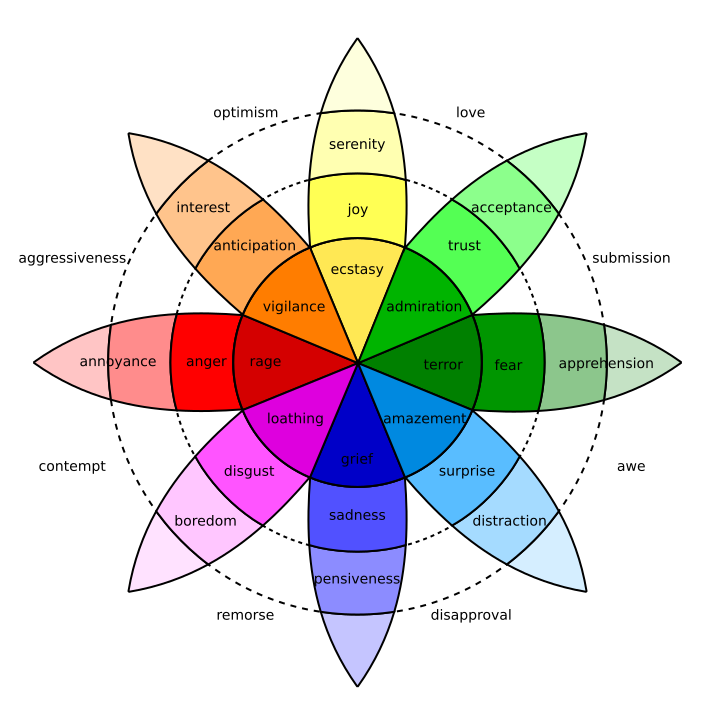
\includegraphics[width=10cm]{figures/plutchik-wheel.png}
\fcmfcaption{Koło emocji Plutchika \cite{plutchik1982psychoevolutionary}.}\label{rys:plutchik_wheel}
\end{figure}

Podsumowując wymienione modele emocji możemy wydzielić dwa główne typy: kategoryczne oraz wymiarowe. Modele wymiarowe mapują emocję w sposób ciągły na wektory. Modele kategoryczne klasyfikują emocję do konkretnej emocji dyskretnej, np. jednej z wybranego modelu emocji Ekmana lub Plutchika. Modele kategoryczne mają pewne wady. Jedną z nich jest brak możliwości opisania innych emocji oraz utrudnione opisywanie emocji złożonej z kilku różnych podtypów zdefiniowanych w dyskretnym modelu. Drugą wadą jest brak możliwości porównywania emocji, co umożliwiłby model wymiarowy, za pomocą porównywania dwóch wektorów. Wybór odpowiedniego modelu emocji nie jest łatwy, a jednocześnie jest bardzo ważnym elementem do późniejszej klasyfikacji emocji. Decydując się na kategoryczny typ emocji, z jednej strony mamy prosty model Ekmana który nie jest w stanie zamodelować złożonych emocji. Z drugiej strony w modelu Plutchika może być bardzo trudno rozróżnić drobnoziarniste emocje od siebie. Wybór ten należy zatem dokonać mając na uwadze wielkość oraz jakość zbioru danych.

\section{Głębokie uczenie}

W przetwarzaniu języka naturalnego z użyciem głębokich sieci neuronowych coraz częściej używane są techniki transferu wiedzy (ang. \textit{transfer learning}) oraz adaptacji domenowej. Model języka jest kluczowym elementem do zastosowania powyższych technik. Umożliwia on przewidzenie kontekstu w jakim dane słowo znajduje się w zdaniu i na tej podstawie umożliwia odkryć jego prawdziwy sens. Jest uważany za bardzo istotny element w dziedzinie \textit{NLP}, który stanowi podstawę do wszelkich zastosowań przetwarzania języka naturalnego. Najważniejsze jego cechy to zrozumienie długofalowych zależności i hierarchicznej struktury tekstu, a największe zalety to otwarte i wolne zasoby do jego stworzenia. Jest tworzony za pomocą nienadzorowanego procesu uczenia, który potrzebuje tylko korpusu nieoznakowanego tekstu.

Znakomitym przykładem użycia transferu wiedzy za pomocą wielokrotnego uczenia modelu języka jest metoda \textit{ULMFIT} \cite{howard2018universal} (ang. \textit{Universal Language Model Fine-tuning for Text Classification}, która może być zastosowana do każdego zadania w NLP. Zastosowane są w niej techniki, które są kluczowe dla dostrojenia modelu językowego. Używane są w niej 3 warstwy sieci neuronowej wykorzystującej komórki LSTM (ang. \textit{Long Short-Term Memory}), które w przeciwieństwie do standardowych komórek sieci neuronowych, posiadają połączenia zwrotne, umożliwiające zapamiętanie sąsiednich stanów w sieci. Dodatkowo zastosowana jest technika przerywania (ang. \textit{dropout}) niwelująca problem przeuczania. Cały etap nauki w metodzie \textit{ULMFIT} składa się z 3 etapów zaprezentowanych na rysunku \ref{rys:ulmfit}. Na początku następuje szkolenie wstępne modelu językowego na dowolnym korpusie, następnie dostrojenie modelu językowego na zadaniu docelowym i na końcu dostrojenie klasyfikatora na zadaniu docelowym. Dzięki zastosowaniu tych technik możliwe jest wyuczenie wstępne modelu języka na dowolnych danych, (np. korpus Wikipedii) a następnie wykorzystanie tego wstępnie wyuczonego modelu na zadaniu docelowym. Na podobnej zasadzie działają dzisiejsze najbardziej wyrafinowane architektury głębokich sieci neuronowych w zastosowaniu przetwarzania języka naturalnego nazywane aktualnym stanem techniki (ang. \textit{state of the art}).

\begin{figure}[t]
\centering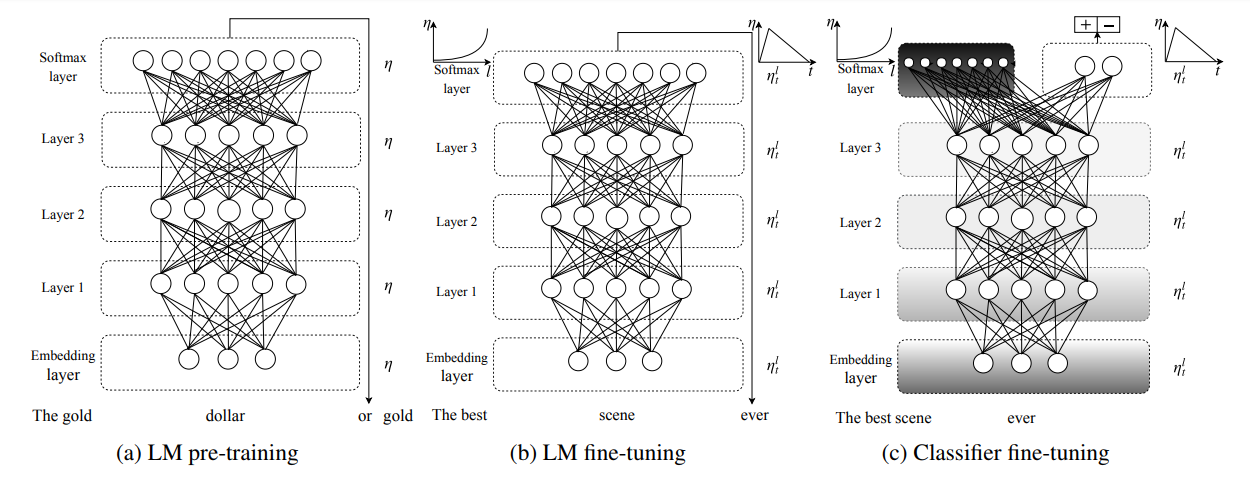
\includegraphics[width=\textwidth]{figures/ulmfit.png}
\fcmfcaption{3 etapy nauki modelu języka (ang. \textit{LM}) w metodzie ULMFIT \cite{howard2018universal}.}\label{rys:ulmfit}
\end{figure}
\chapter{Analiza eksploracyjna}

Rozdziały dokumentujące pracę własną studenta: opisujące ideę, sposób lub metodę 
rozwiązania postawionego problemu oraz rozdziały opisujące techniczną stronę rozwiązania 
--- dokumentacja techniczna, przeprowadzone testy, badania i uzyskane wyniki. 

Praca musi zawierać elementy pracy własnej autora adekwatne do jego wiedzy praktycznej uzyskanej w
okresie studiów. Za pracę własną autora można uznać np.: stworzenie aplikacji informatycznej lub jej
fragmentu, zaproponowanie algorytmu rozwiązania problemu szczegółowego, przedstawienie projektu 
np.~systemu informatycznego lub sieci komputerowej, analizę i ocenę nowych technologii lub rozwiązań
informatycznych wykorzystywanych w przedsiębiorstwach, itp. 

Autor powinien zadbać o właściwą dokumentację pracy własnej obejmującą specyfikację założeń i 
sposób realizacji poszczególnych zadań
wraz z ich oceną i opisem napotkanych problemów. W przypadku prac o charakterze 
projektowo-implementacyjnym, ta część pracy jest zastępowana dokumentacją techniczną i użytkową systemu. 

W pracy \textbf{nie należy zamieszczać całego kodu źródłowego} opracowanych programów. Kod źródłowy napisanych
programów, wszelkie oprogramowanie wytworzone i wykorzystane w pracy, wyniki przeprowadzonych
eksperymentów powinny być umieszczone np. na płycie CD, stanowiącej dodatek do pracy.

\section*{Styl tekstu}

Należy\footnote{Uwagi o stylu pochodzą częściowo ze stron prof. Macieja Drozdowskiego~\cite{zhong2019knowledgeenriched}.} 
stosować formę bezosobową, tj.~\emph{w pracy rozważono ......, 
w ramach pracy zaprojektowano ....}, a nie: \emph{w pracy rozważyłem, w ramach pracy zaprojektowałem}. 
Odwołania do wcześniejszych fragmentów tekstu powinny mieć następującą postać: ,,Jak wspomniano wcześniej, ....'', 
,,Jak wykazano powyżej ....''. Należy unikać długich zdań. 

Niedopuszczalne są zwroty używane w języku potocznym. W pracy należy używać terminologii informatycznej, która ma 
sprecyzowaną treść i znaczenie. 

Niedopuszczalne jest pisanie pracy metodą \emph{cut\&paste}, bo jest to plagiat i dowód intelektualnej indolencji autora.
Dane zagadnienie należy opisać własnymi słowami. Zawsze trzeba powołać się na zewnętrzne źródła. 

\chapter{Zbiory danych}
\chapter{Przetwarzanie danych}
\chapter{Budowa modeli}
\chapter{Ewaluacja modeli}
\chapter{Zakończenie}

Zakończenie pracy zwane również Uwagami końcowymi lub Podsumowaniem powinno zawierać ustosunkowanie
się autora do zadań wskazanych we wstępie do pracy, a w szczególności do celu i zakresu pracy oraz
porównanie ich z faktycznymi wynikami pracy. Podejście takie umożliwia jasne określenie stopnia
realizacji założonych celów oraz zwrócenie uwagi na wyniki osiągnięte przez autora w ramach jego
samodzielnej pracy.

Integralną częścią pracy są również dodatki, aneksy i załączniki zawierające stworzone w ramach pracy programy, aplikacje i projekty.

%--------------------------------------
% Literatura
%--------------------------------------

\bibliographystyle{plain}{\raggedright\sloppy\small\bibliography{bibliografia}}

%--------------------------------------
% Dodatki
%--------------------------------------

% EDIT: Te 3 linijki nie były zakomentowane, te nowe page może trzeba bedzie odkomentować
% \cleardoublepage\appendix%
% \newpage
% \chapter{Płyta CD}

Płyta CD z elektroniczną wersją pracy, stworzonym projektem oraz danymi wejściowymi.

%--------------------------------------
% Informacja o prawach autorskich
%--------------------------------------

\ppcolophon

\end{document}
